\documentclass[tikz]{standalone}
\usetikzlibrary{calc,through,intersections,backgrounds,patterns}
\begin{document}
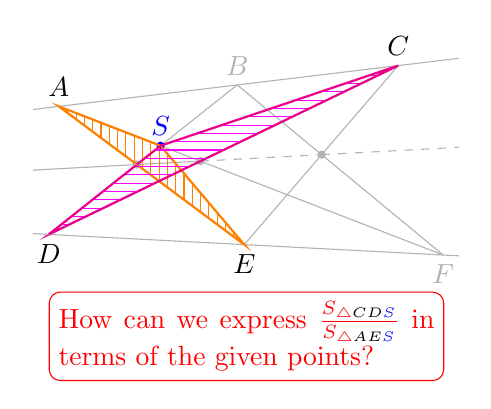
\begin{tikzpicture}
  \def\A{$A$}
  \def\B{\textcolor{hidden}{$B$}}
  \def\C{$C$}
  \def\D{$D$}
  \def\E{$E$}
  \def\F{\textcolor{hidden}{$F$}}
  \def\P{\textcolor{hidden}{$P$}}
  \def\Q{\textcolor{hidden}{$Q$}}
  \def\R{\textcolor{hidden}{$R$}}
  \colorlet{hidden}{black!30}

  % draw the given points first
  \coordinate [label={[name=lblA]above:\A}]
    (A) at ($ (0.2,1.8) + .1*(rand,rand) $);
  \coordinate [label=above:\B] (B) at ($ (2.3,2.2) + .1*(rand,rand) $);
  \coordinate [label={[name=lblC]above:\C}]
    (C) at ($ (A) ! 2+.1*rand ! (B) $);
  \draw [color=hidden] (A) -- (B) -- (C);
  \coordinate [label={[name=lblD]below:\D}]
    (D) at ($ (0,0.3) + .1*(rand,rand) $);
  \coordinate [label=below:\E] (E) at ($ (2.5,0.2) + .1*(rand,rand) $);
  \coordinate [label={[name=lblF]below:\F}]
    (F) at ($ (D) ! 2+.1*rand ! (E) $);
  \draw [color=hidden] (D) -- (E) -- (F);

  % Draw the segments
  \draw [color=hidden,name path=A--E] (A) -- (E);
  \draw [color=hidden,name path=B--D] (B) -- (D);
  \draw [color=hidden,name path=B--F] (B) -- (F);
  \draw [color=hidden,name path=C--E] (C) -- (E);
  \draw [color=hidden,name path=A--F] (A) -- (F);
  \draw [color=hidden,name path=C--D] (C) -- (D);

  % Get the intersection points
  \path [name intersections={of=A--E and B--D, by={P}}];
  \path [name intersections={of=B--F and C--E, by={R}}];
  \path [name intersections={of=A--F and C--D, by={Q}}];

  % Colour the intersection points
  \foreach \pt in {P,Q,R}
    \fill [hidden] (\pt) circle (1.5pt);

  % Point out the problem
  \draw [hidden] (P) -- (Q);
  \draw [hidden,dashed] (Q) -- (R);

  % Define the new point and reveal the triangle
  \def\S{\textcolor{blue}{$S$}}
  \path [name intersections={of=A--F and B--D, by={[label=above:\S]S}}];
  \fill [blue] (S) circle (1.5pt);
  \draw [color=orange,thick,pattern=vertical lines,pattern color=orange]
    (A) -- (E) -- (S) -- cycle;
  \draw [color=magenta,thick,pattern=horizontal lines,pattern color=magenta]
    (C) -- (D) -- (S) -- cycle;

  % Text below
  % Help identify the positions of points
  %\coordinate [label=$O$] (O) at (0,0);
  %\fill [blue] (O) circle (1pt);
  %\draw [help lines,step=.1] (-.5,-.5) grid (5,3);
  \path let \p1=(lblD.base), % lowest point of text label
            \p2=(lblF.base),
            \p3=(lblA.base),
            \p4=(lblC.base),
	    % expr: veclen needed, default inner sep is .3333em
            \n3 = {(max(veclen(\x1 - \x2,0),veclen(\x3 - \x4,0)))
	      -2*.3333em},
            \n4 = {(min(\y1,\y2))-1mm} % expr: 1cm is the basic unit
         in
    node [color=red,anchor=north west,draw,text width=\n3,align=justify,rounded corners]
    (T) at (\x1,\n4)
    % expr: red needed to avoid change the color change to black
    {\color{red}How can we express
    $\frac{S_{\triangle {\color{black}CD}{\color{blue}S}}}
      {S_{\triangle {\color{black}AE}{\color{blue}S}}}$ in terms of
      the given points?};
    %\fill [green] (lblD) circle (1pt);
    %\fill [green] (lblF) circle (1pt);
    %\fill [red] (T.north west) circle (1pt);

  % Set the visible area of the figure for the next part
  % The following 2 parts are put to the bottom to avoid problems in
  % filling the area with patterns.
  \clip
    let \p1=(A),
        \p2=(C),
        \p3=(D),
        \p4=(F),
	\n5={(min(\x1,\x2,\x3,\x4))-2mm},
	\n6={(min(\y1,\y2,\y3,\y4))-2mm},
	\n7={(max(\x1,\x2,\x3,\x4))+2mm},
	\n8={(max(\y1,\y2,\y3,\y4))+2mm}
    in
      (\n5,\n6) rectangle (\n7,\n8);

  % Extend the given segments so that they look like lines
  \draw [color=hidden] (A) -- ($ (A) ! -1 ! (B) $);
  \draw [color=hidden] (C) -- ($ (A) ! 3 ! (B) $);
  \draw [color=hidden] (D) -- ($ (D) ! -1 ! (E) $);
  \draw [color=hidden] (F) -- ($ (D) ! 3 ! (E) $);
  \draw [hidden] ($ (P) ! -5 ! (Q) $) -- (P);
  \draw [hidden,dashed] (R) -- ($ (P) ! 9 ! (Q) $);
\end{tikzpicture}
\end{document}
